\newpage
\subsection{QuizziPedia::Front-End::QML}


\begin{figure} [ht]
	\centering
	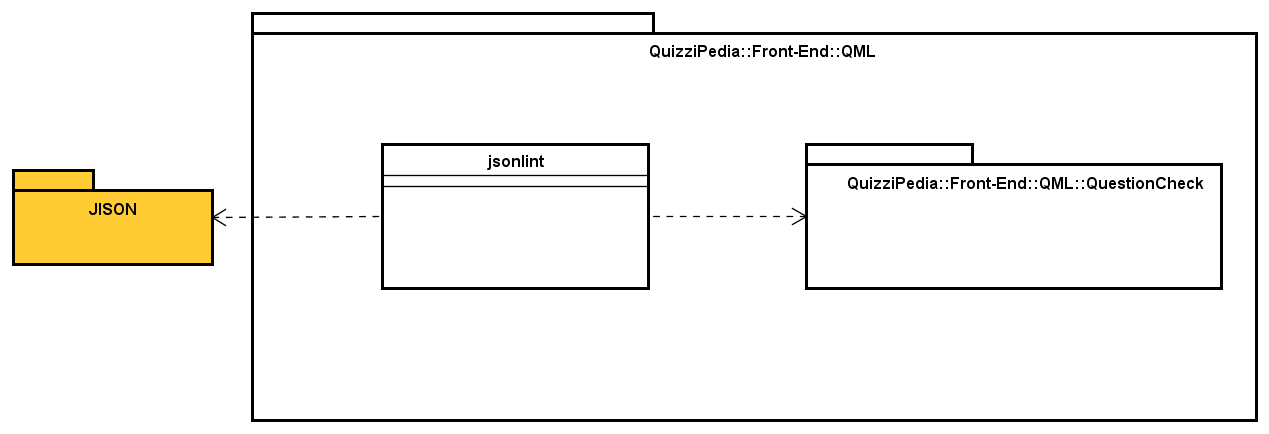
\includegraphics[scale=0.42]{UML/Package/QuizziPedia_Front-End_QML.png}
	\caption{QuizziPedia::Front-End::QML}
\end{figure} \FloatBarrier

\subsubsection{Informazioni generali}
\begin{itemize}
	\item \textbf{Descrizione}: \textit{package\ped{G}} che contiene i componenti individuati per la parte realizzazione del linguaggio di \textit{markup\ped{G}} \textit{QML\ped{G}} dell'applicazione;
	\item \textbf{Padre}: \texttt{Front-End};
	\item \textbf{Interazione con altri componenti}:
	\begin{itemize}
		\item \texttt{Controller}: \textit{package\ped{G}} che contiene le classi controller individuate;
		\item \texttt{View}: \textit{package\ped{G}} che contiene le classi view individuate.
	\end{itemize} 
\end{itemize}
\subsubsection{Classi}

\paragraph[QuizziPedia::Front-End::QML::jsonlint]{QuizziPedia::Front-End::QML::jsonlint}
\begin{figure} [ht]
	\centering
	\includegraphics[scale=0.80]{UML/Classi/Front-End/QuizziPedia_Front-end_QML_jsonlint.png}
	\caption{QuizziPedia::Front-End::QML::jsonlint}
\end{figure} \FloatBarrier
\begin{itemize}
	\item \textbf{Descrizione}: questa classe implementa il \textit{parser\ped{G}} per il controllo della grammatica del \textit{QML\ped{G}};
	\item \textbf{Utilizzo}: fornisce le funzionalità per controllare la validità sintattica del codice \textit{QML\ped{G}};
	\item \textbf{Relazioni con altre classi}:
	\begin{itemize}
		\item \textbf{IN} \texttt{EditorQMLview}: \textit{view\ped{G}} contenente l'\textit{editor\ped{G}} \textit{QML\ped{G}} per la creazione di domande personalizzate,
		permette ad un utente di creare domande personalizzate attraverso la scrittura del codice \textit{QML\ped{G}} direttamente nell'\textit{editor\ped{G}} di testo presente nella \textit{view\ped{G}};
		\item \textbf{OUT} \texttt{CheckQML} : questa classe contiene i metodi per controllare la validità semantica del codice \textit{QML\ped{G}}.
	\end{itemize}
	\item \textbf{Metodi}:
	\begin{itemize}
		\item \texttt{+} \texttt{jsonlint(body : String)} \\ 
		Questo metodo controlla la validità sintattica del codice \textit{QML\ped{G}}, fa uso della classe \texttt{json2} messa a disposizione dalla libreria \textit{JISON\ped{G}}. \\
		\textbf{Parametri}:
		\begin{itemize}
			\item \texttt{body : String} \\
			Parametro contenente il codice QML scritto dall'utente nell'editor di testo.
		\end{itemize}
	\end{itemize}
\end{itemize}


\newpage
\subsubsection{QuizziPedia::Front-End::QML::QuestionCheck}


\begin{figure} [ht]
	\centering
	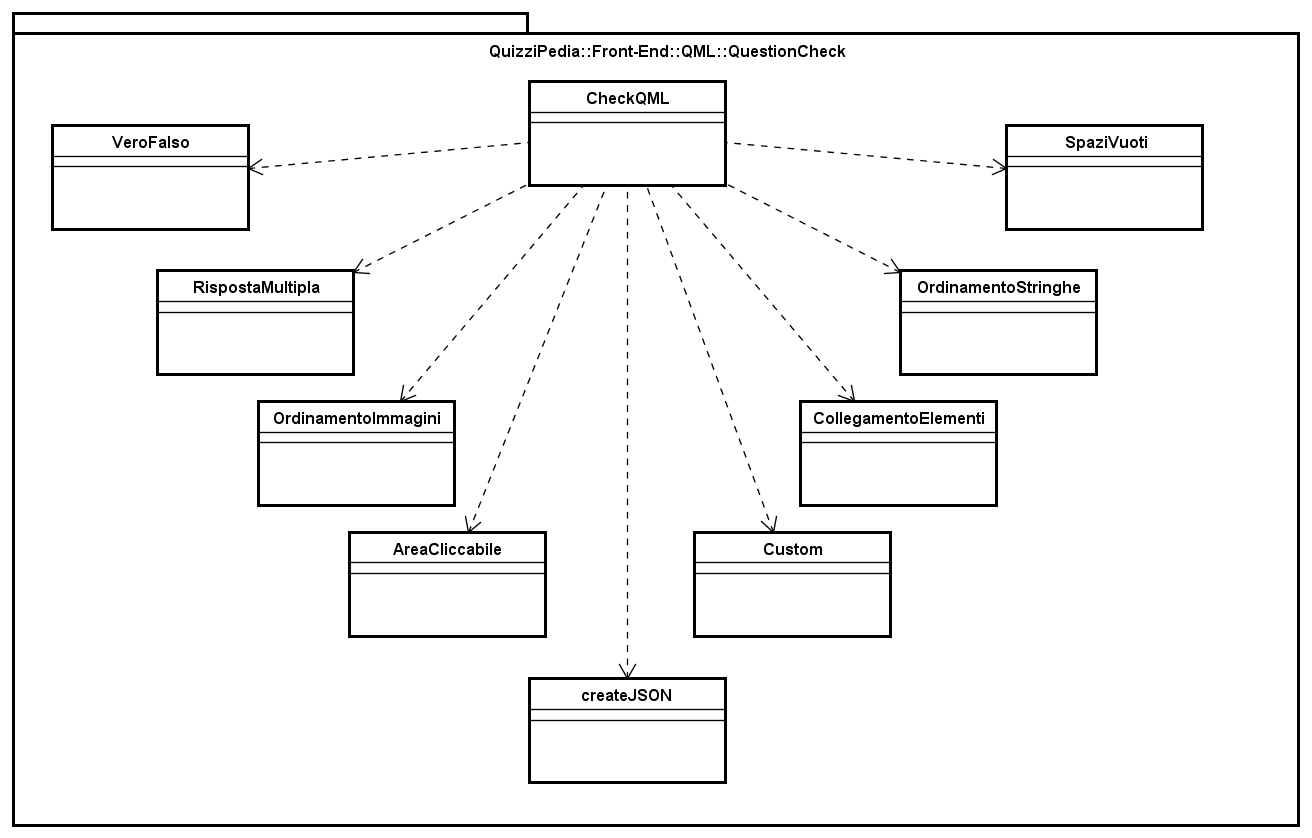
\includegraphics[scale=0.42]{UML/Package/QuizziPedia_Front-End_QML_QuestionCheck.png}
	\caption{QuizziPedia::Front-End::QML::QuestionCheck}
\end{figure} \FloatBarrier

\subsubsection{Informazioni generali}
\begin{itemize}
	\item \textbf{Descrizione}: \textit{package\ped{G}} che contiene i componenti individuati per la verifica semantica del linguaggio di \textit{markup\ped{G}} \textit{QML\ped{G}} dell'applicazione;
	\item \textbf{Interazione con altri componenti}:
	\begin{itemize}
		\item \texttt{Models}: \textit{package\ped{G}} che contiene le classi model individuate;
		\item \texttt{Services}: \textit{package\ped{G}} che contiene le classi services individuate.
	\end{itemize} 
\end{itemize}
\subsubsection{Classi}

\paragraph[QuizziPedia::Front-End::QML:: \\ QuestionCheck::CheckQML]{QuizziPedia::Front-End::QML::QuestionCheck::CheckQML}
\begin{figure} [ht]
	\centering
	\includegraphics[scale=0.32]{UML/Classi/Front-End/QuizziPedia_Front-end_QML_QuestionCheck_CheckQML.png}
	\caption{QuizziPedia::Front-End::QML::QuestionCheck::CheckQML}
\end{figure} \FloatBarrier
\begin{itemize}
	\item \textbf{Descrizione}: questa classe implementa il metodo che permette di controllare la validità semantica del codice \textit{QML\ped{G}};
	\item \textbf{Utilizzo}: fornisce le funzionalità per controllare la validità semantica del codice \textit{QML\ped{G}};
	\item \textbf{Relazioni con altre classi}:
	\begin{itemize}
		\item \textbf{IN} \texttt{EditorQMLcontroller}: questa classe permette di gestire la creazione e la modifica di domande create tramite editor QML;		
		\item \textbf{OUT} \texttt{AreaCliccabile}: usata per controllare la validità semantica del codice \textit{QML\ped{G}} nello specifico caso di tipologia "AreaCliccabile";
		\item \textbf{OUT} \texttt{CollegamentoElementi}: usata per controllare la validità semantica del codice \textit{QML\ped{G}} nello specifico caso di tipologia "CollegamentoElementi";
		\item \textbf{OUT} \texttt{Custom}: usata per controllare la validità semantica del codice \textit{QML\ped{G}} nello specifico caso di tipologia "Custom";
		\item \textbf{OUT} \texttt{OrdinamentoImmagini}: usata per controllare la validità semantica del codice \textit{QML\ped{G}} nello specifico caso di tipologia "OrdinamentoImmagini";
		\item \textbf{OUT} \texttt{OrdinamentoStringhe}: usata per controllare la validità semantica del codice \textit{QML\ped{G}} nello specifico caso di tipologia "OrdinamentoStringhe";
		\item \textbf{OUT} \texttt{SpaziVuoti}: usata per controllare la validità semantica del codice \textit{QML\ped{G}} nello specifico caso di tipologia "SpaziVuoti";
		\item \textbf{OUT} \texttt{RispostaMultipla}: usata per controllare la validità semantica del codice \textit{QML\ped{G}} nello specifico caso di tipologia "RispostaMultipla";
		\item \textbf{OUT} \texttt{VeroFalso}: usata per controllare la validità semantica del codice \textit{QML\ped{G}} nello specifico caso di tipologia "VeroFalso";
		\item \textbf{OUT} \texttt{CreateJSON}:
	\end{itemize}
	\item \textbf{Metodi}:
	\begin{itemize}
		\item \texttt{+} \texttt{controlloQML(req : JSON, res : JSON, topics : String)} \\ 
		Questo metodo controlla la validità sintattica del codice \textit{QML\ped{G}}, fa uso della classe \texttt{json2} messa a disposizione dalla libreria \textit{JISON\ped{G}}. \\
		\textbf{Parametri}:
		\begin{itemize}
			\item \texttt{req : JSON} \\
			Parametro contenente il codice QML scritto dall'utente nell'editor di testo e sintatticamente valido;
			\item \texttt{res : JSON} \\
			Parametro che contiene il JSON specifico per la domanda da creare o un JSON con un messaggio d'errore;
			\item \texttt{topics : String} \\
			Parametro che indica l'argomento della domanda da creare, necessario per eseguire i giusti controlli semantici nel corpo del codice \textit{QML\ped{G}}.
		\end{itemize}
	\end{itemize}
\end{itemize}


\paragraph[QuizziPedia::Front-End::QML:: \\ QuestionCheck::AreaCliccabile]{QuizziPedia::Front-End::QML::QuestionCheck::AreaCliccabile}
\begin{figure} [ht]
	\centering
	\includegraphics[scale=0.32]{UML/Classi/Front-End/QuizziPedia_Front-end_QML_QuestionCheck_AreaCliccabile.png}
	\caption{QuizziPedia::Front-End::QML::QuestionCheck::AreaCliccabile}
\end{figure} \FloatBarrier
\begin{itemize}
	\item \textbf{Descrizione}: questa classe implementa il metodo che permette di controllare la validità semantica del codice \textit{QML\ped{G}} relativo alla tipologia di domanda "AreaCliccabile";
	\item \textbf{Utilizzo}: usata per controllare la validità semantica del codice \textit{QML\ped{G}} nello specifico caso di tipologia "AreaCliccabile";
	\item \textbf{Relazioni con altre classi}:
	\begin{itemize}
		\item \textbf{IN} \texttt{CheckQML}: classe che fornisce le funzionalità per controllare la validità semantica del codice \textit{QML\ped{G}}.
	\end{itemize}
	\item \textbf{Metodi}:
	\begin{itemize}
		\item \texttt{+} \texttt{areaCliccabile(req : JSON, res : JSON)} \\
		 Questo metodo permette di controllare la semantica del codice \textit{QML\ped{G}}, restituisce un JSON con la domanda valida oppure un JSON contenente un messaggio d'errore. \\
		\textbf{Parametri}:
		\begin{itemize}
			\item \texttt{req : JSON} \\
			Parametro contenente il codice QML scritto dall'utente nell'editor di testo e sintatticamente valido;
			\item \texttt{res : JSON} \\
			Parametro che contiene il JSON specifico per la domanda da creare o un JSON con un messaggio d'errore;
		\end{itemize}
	\end{itemize}
\end{itemize}


\paragraph[QuizziPedia::Front-End::QML:: \\ QuestionCheck::Collegamentoelementi]{QuizziPedia::Front-End::QML::QuestionCheck::CollegamentoElementi}
\begin{figure} [ht]
	\centering
	\includegraphics[scale=0.32]{UML/Classi/Front-End/QuizziPedia_Front-end_QML_QuestionCheck_CollegamentoElementi.png}
	\caption{QuizziPedia::Front-End::QML::QuestionCheck::CollegamentoElementi}
\end{figure} \FloatBarrier
\begin{itemize}
	\item \textbf{Descrizione}: questa classe implementa il metodo che permette di controllare la validità semantica del codice \textit{QML\ped{G}} relativo alla tipologia di domanda "CollegamentoElementi";
	\item \textbf{Utilizzo}: usata per controllare la validità semantica del codice \textit{QML\ped{G}} nello specifico caso di tipologia "CollegamentoElementi";
	\item \textbf{Relazioni con altre classi}:
	\begin{itemize}
		\item \textbf{IN} \texttt{CheckQML}: classe che fornisce le funzionalità per controllare la validità semantica del codice \textit{QML\ped{G}}.
	\end{itemize}
	\item \textbf{Metodi}:
	\begin{itemize}
		\item \texttt{+} \texttt{collegamentoElementi(req : JSON, res : JSON)} \\
		Questo metodo permette di controllare la semantica del codice \textit{QML\ped{G}}, restituisce un JSON con la domanda valida oppure un JSON contenente un messaggio d'errore. \\
		\textbf{Parametri}:
		\begin{itemize}
			\item \texttt{req : JSON} \\
			Parametro contenente il codice QML scritto dall'utente nell'editor di testo e sintatticamente valido;
			\item \texttt{res : JSON} \\
			Parametro che contiene il JSON specifico per la domanda da creare o un JSON con un messaggio d'errore;
		\end{itemize}
	\end{itemize}
\end{itemize}


\paragraph[QuizziPedia::Front-End::QML:: \\ QuestionCheck::OrdinamentoImmagini]{QuizziPedia::Front-End::QML::QuestionCheck::OrdinamentoImmagini}
\begin{figure} [ht]
	\centering
	\includegraphics[scale=0.80]{UML/Classi/Front-End/QuizziPedia_Front-end_QML_QuestionCheck_OrdinamentoImmagini.png}
	\caption{QuizziPedia::Front-End::QML::QuestionCheck::OrdinamentoImmagini}
\end{figure} \FloatBarrier
\begin{itemize}
	\item \textbf{Descrizione}: questa classe implementa il metodo che permette di controllare la validità semantica del codice \textit{QML\ped{G}} relativo alla tipologia di domanda "OrdinamentoImmagini";
	\item \textbf{Utilizzo}: usata per controllare la validità semantica del codice \textit{QML\ped{G}} nello specifico caso di tipologia "OrdinamentoImmagini";
	\item \textbf{Relazioni con altre classi}:
	\begin{itemize}
		\item \textbf{IN} \texttt{CheckQML}: classe che fornisce le funzionalità per controllare la validità semantica del codice \textit{QML\ped{G}}.
	\end{itemize}
	\item \textbf{Metodi}:
	\begin{itemize}
		\item \texttt{+} \texttt{ordinamentoImmagini(req : JSON, res : JSON)} \\
		Questo metodo permette di controllare la semantica del codice \textit{QML\ped{G}}, restituisce un JSON con la domanda valida oppure un JSON contenente un messaggio d'errore. \\
		\textbf{Parametri}:
		\begin{itemize}
			\item \texttt{req : JSON} \\
			Parametro contenente il codice QML scritto dall'utente nell'editor di testo e sintatticamente valido;
			\item \texttt{res : JSON} \\
			Parametro che contiene il JSON specifico per la domanda da creare o un JSON con un messaggio d'errore;
		\end{itemize}
	\end{itemize}
\end{itemize}
\paragraph[QuizziPedia::Front-End::QML:: \\ QuestionCheck::OrdinamentoStringhe]{QuizziPedia::Front-End::QML::QuestionCheck::OrdinamentoStringhe}
\begin{figure} [ht]
	\centering
	\includegraphics[scale=0.80]{UML/Classi/Front-End/QuizziPedia_Front-end_QML_QuestionCheck_OrdinamentoStringhe.png}
	\caption{QuizziPedia::Front-End::QML::QuestionCheck::OrdinamentoStringhe}
\end{figure} \FloatBarrier
\begin{itemize}
	\item \textbf{Descrizione}: questa classe implementa il metodo che permette di controllare la validità semantica del codice \textit{QML\ped{G}} relativo alla tipologia di domanda "OrdinamentoStringhe";
	\item \textbf{Utilizzo}: usata per controllare la validità semantica del codice \textit{QML\ped{G}} nello specifico caso di tipologia "OrdinamentoStringhe";
	\item \textbf{Relazioni con altre classi}:
	\begin{itemize}
		\item \textbf{IN} \texttt{CheckQML}: classe che fornisce le funzionalità per controllare la validità semantica del codice \textit{QML\ped{G}}.
	\end{itemize}
	\item \textbf{Metodi}:
	\begin{itemize}
		\item \texttt{+} \texttt{ordinamentoStringhe(req : JSON, res : JSON)} \\
		Questo metodo permette di controllare la semantica del codice \textit{QML\ped{G}}, restituisce un JSON con la domanda valida oppure un JSON contenente un messaggio d'errore. \\
		\textbf{Parametri}:
		\begin{itemize}
			\item \texttt{req : JSON} \\
			Parametro contenente il codice QML scritto dall'utente nell'editor di testo e sintatticamente valido;
			\item \texttt{res : JSON} \\
			Parametro che contiene il JSON specifico per la domanda da creare o un JSON con un messaggio d'errore;
		\end{itemize}
	\end{itemize}
\end{itemize}


\paragraph[QuizziPedia::Front-End::QML:: \\ QuestionCheck::RispostaMultipla]{QuizziPedia::Front-End::QML::QuestionCheck::RispostaMultipla}
\begin{figure} [ht]
	\centering
	\includegraphics[scale=0.32]{UML/Classi/Front-End/QuizziPedia_Front-end_QML_QuestionCheck_RispostaMultipla.png}
	\caption{QuizziPedia::Front-End::QML::QuestionCheck::RispostaMultipla}
\end{figure} \FloatBarrier
\begin{itemize}
	\item \textbf{Descrizione}: questa classe implementa il metodo che permette di controllare la validità semantica del codice \textit{QML\ped{G}} relativo alla tipologia di domanda "RispostaMultipla";
	\item \textbf{Utilizzo}: usata per controllare la validità semantica del codice \textit{QML\ped{G}} nello specifico caso di tipologia "RispostaMultipla";
	\item \textbf{Relazioni con altre classi}:
	\begin{itemize}
		\item \textbf{IN} \texttt{CheckQML}: classe che fornisce le funzionalità per controllare la validità semantica del codice \textit{QML\ped{G}}.
	\end{itemize}
	\item \textbf{Metodi}:
	\begin{itemize}
		\item \texttt{+} \texttt{rispostaMultipla(req : JSON, res : JSON)} \\
		Questo metodo permette di controllare la semantica del codice \textit{QML\ped{G}}, restituisce un JSON con la domanda valida oppure un JSON contenente un messaggio d'errore. \\
		\textbf{Parametri}:
		\begin{itemize}
			\item \texttt{req : JSON} \\
			Parametro contenente il codice QML scritto dall'utente nell'editor di testo e sintatticamente valido;
			\item \texttt{res : JSON} \\
			Parametro che contiene il JSON specifico per la domanda da creare o un JSON con un messaggio d'errore;
		\end{itemize}
	\end{itemize}
\end{itemize}


\paragraph[QuizziPedia::Front-End::QML:: \\ QuestionCheck::SpaziVuoti]{QuizziPedia::Front-End::QML::QuestionCheck::SpaziVuoti}
\begin{figure} [ht]
	\centering
	\includegraphics[scale=0.80]{UML/Classi/Front-End/QuizziPedia_Front-end_QML_QuestionCheck_SpaziVuoti.png}
	\caption{QuizziPedia::Front-End::QML::QuestionCheck::SpaziVuoti}
\end{figure} \FloatBarrier
\begin{itemize}
	\item \textbf{Descrizione}: questa classe implementa il metodo che permette di controllare la validità semantica del codice \textit{QML\ped{G}} relativo alla tipologia di domanda "SpaziVuoti";
	\item \textbf{Utilizzo}: usata per controllare la validità semantica del codice \textit{QML\ped{G}} nello specifico caso di tipologia "SpaziVuoti";
	\item \textbf{Relazioni con altre classi}:
	\begin{itemize}
		\item \textbf{IN} \texttt{CheckQML}: classe che fornisce le funzionalità per controllare la validità semantica del codice \textit{QML\ped{G}}.
	\end{itemize}
	\item \textbf{Metodi}:
	\begin{itemize}
		\item \texttt{+} \texttt{riempimentoSpaziVuoti(req : JSON, res : JSON)} \\
		Questo metodo permette di controllare la semantica del codice \textit{QML\ped{G}}, restituisce un JSON con la domanda valida oppure un JSON contenente un messaggio d'errore. \\
		\textbf{Parametri}:
		\begin{itemize}
			\item \texttt{req : JSON} \\
			Parametro contenente il codice QML scritto dall'utente nell'editor di testo e sintatticamente valido;
			\item \texttt{res : JSON} \\
			Parametro che contiene il JSON specifico per la domanda da creare o un JSON con un messaggio d'errore;
		\end{itemize}
	\end{itemize}
\end{itemize}


\paragraph[QuizziPedia::Front-End::QML:: \\ QuestionCheck::VeroFalso]{QuizziPedia::Front-End::QML::QuestionCheck::veroFalso}
\begin{figure} [ht]
	\centering
	\includegraphics[scale=0.32]{UML/Classi/Front-End/QuizziPedia_Front-end_QML_QuestionCheck_VeroFalso.png}
	\caption{QuizziPedia::Front-End::QML::QuestionCheck::VeroFalso}
\end{figure} \FloatBarrier
\begin{itemize}
	\item \textbf{Descrizione}: questa classe implementa il metodo che permette di controllare la validità semantica del codice \textit{QML\ped{G}} relativo alla tipologia di domanda "VeroFalso";
	\item \textbf{Utilizzo}: usata per controllare la validità semantica del codice \textit{QML\ped{G}} nello specifico caso di tipologia "VeroFalso";
	\item \textbf{Relazioni con altre classi}:
	\begin{itemize}
		\item \textbf{IN} \texttt{CheckQML}: classe che fornisce le funzionalità per controllare la validità semantica del codice \textit{QML\ped{G}}.
	\end{itemize}
	\item \textbf{Metodi}:
	\begin{itemize}
		\item \texttt{+} \texttt{veroFalso(req : JSON, res : JSON)} \\
		Questo metodo permette di controllare la semantica del codice \textit{QML\ped{G}}, restituisce un JSON con la domanda valida oppure un JSON contenente un messaggio d'errore. \\
		\textbf{Parametri}:
		\begin{itemize}
			\item \texttt{req : JSON} \\
			Parametro contenente il codice QML scritto dall'utente nell'editor di testo e sintatticamente valido;
			\item \texttt{res : JSON} \\
			Parametro che contiene il JSON specifico per la domanda da creare o un JSON con un messaggio d'errore;
		\end{itemize}
	\end{itemize}
\end{itemize}




